\documentclass[11pt, a4paper]{report}
\usepackage{etoolbox}
\makeatletter
\patchcmd{\chapter}{\if@openright\cleardoublepage\else\clearpage\fi}{}{}{}
\makeatother
\usepackage[margin=1in]{geometry}
\usepackage[utf8]{inputenc} % Umožňuje psaní českých znaků
\usepackage[czech]{babel}   % Česká lokalizace pro babel
\usepackage{titlesec}
\usepackage{pdfpages}
\usepackage{tabularx}
\usepackage{xcolor}
\titleformat{\chapter}
  {\normalfont\LARGE\bfseries}{\thechapter}{1em}{}
\titlespacing*{\chapter}{0pt}{3.5ex plus 1ex minus .2ex}{2.3ex plus .2ex}
\begin{document}
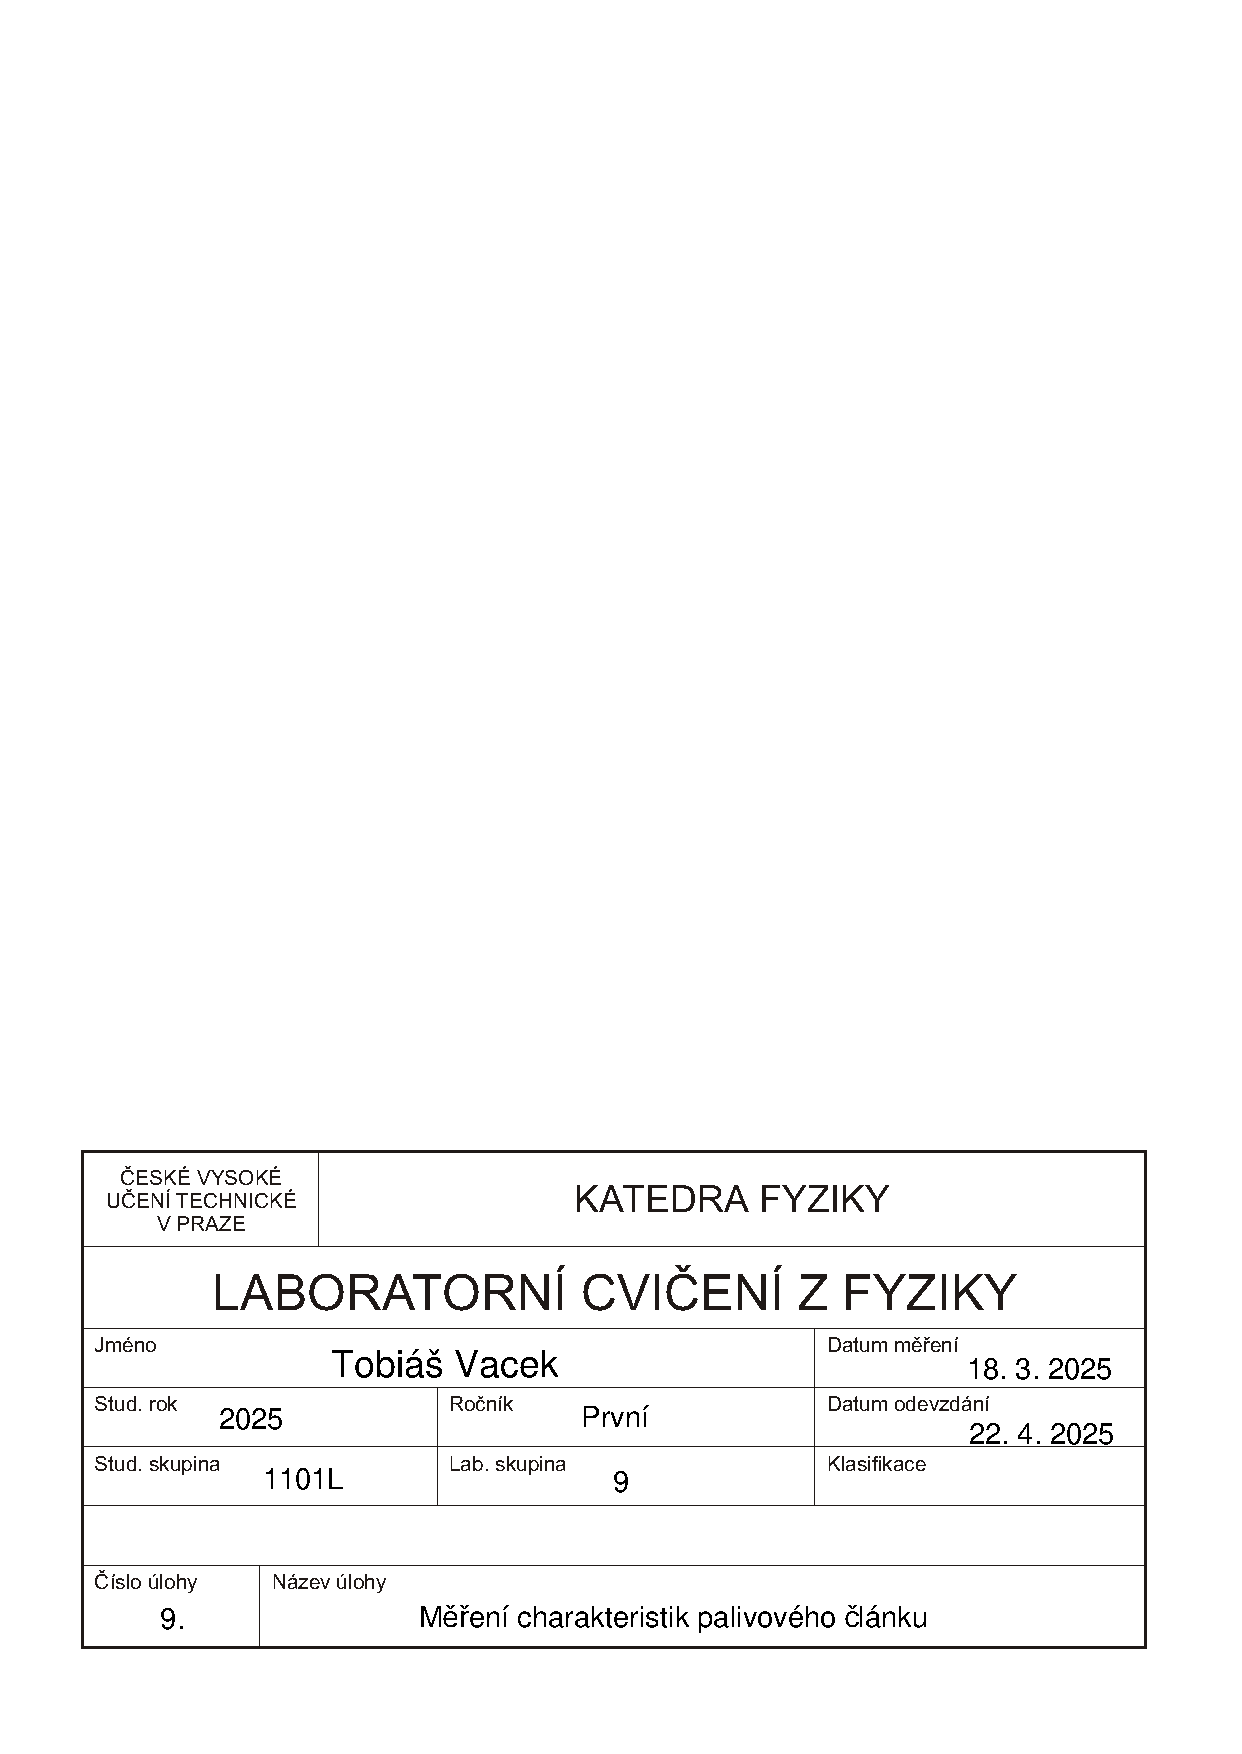
\includepdf{stamp.pdf}
\chapter{Úkol měření}
\begin{enumerate}
	\item Změřte voltampérovou charakteristiku PEM elektrolyzéru, sestrojte graf a extrapolací určete rozkladné napětí elektrolyzéru.
	\item Změřte voltampérovou charakteristiku PEM palivového článku, sestrojte graf a odhadněte maximální výkon, který lze z článku odebírat.
\end{enumerate}

\chapter{Postup měření}
\section{Příprava před měřením}
Elektrolyzér byl při našem příchodu zapojen a naplněn vodou, proto jsme tyto úkony nemuseli dělat.
Začali jsme, proto kontrolou zda není palivový článek zkratován a odpojením všech zatěžovacích rezistorů.
Před zapnutím napájecího zdroje jsme nastavili výstupní napětí a omezovač proudu na nulu.
Zapnuli jsme napajecí zdroj a nastavili na něm napětí 5\,V a omezovač proudu jsme nastavili tak, aby elektrolyzérem protékal maximální proud 2\,A.
Povolili jsme všechna škrtítka na vstupu a výstupu palivového článku a minutu čekali, než se ustálí napětí na elektrolyzéru.

\section{Měření voltampérové charakteristiky elektrolyzéru}
Omezovačem proudu jsme postupně snižovali proud procházející elektrolyzérem, po každé změně bylo nutné minutu počkat, než se ustálí napětí na elektrolyzéru.
Po ustálení jsme si zaznamenali hodnoty napětí a proudu z měřících přístrojů.

\section{Měření voltampérové charakteristiky palivového článku}
Nastavili jsme proud elektrolyzérem opět na maximální povolenou hodnotu 2\,A.
Pro zajištění stabilních provozních podmínek jsme palivový článek na dobu pěti minut zatížili odporem 2\,$\Omega$.
Po pěti minutách jsme zátěž odpojili a změřili napětí na prázdno.
Nasledně jsme článek postupně zatěžovali různými kombinacemi odporů.
Kombinace jsme měnili sestupně.

\chapter{Seznam použitých přístrojů}


\begin{center}
	\begin{tabularx}{\textwidth}{|>{\centering\arraybackslash}X
		|>{\centering\arraybackslash}X
		|>{\centering\arraybackslash}X
		|>{\centering\arraybackslash}X
		|>{\centering\arraybackslash}X|}
		\hline
		\textbf{Počet} & \textbf{Pomůcka}    & \textbf{číslo} & \textbf{Přesnost}        & \textbf{Rozsah} \\
		\hline
		3              & ampérmetr           & MY-65          & \pm 2\,\% (\pm 5 digitů) & 10\,A           \\
		\hline
		2              & voltmetr            & MY-65          & \pm0,5\,\% (\pm1 digit)  & 20\,V           \\
		\hline
		1              & voltmetr            & MY-65          & \pm0,5\,\% (\pm1 digit)  & 2\,V            \\
		\hline
		2              & Zatěžovací rezistor & -----          &                          & 10\,Ω, 20\,Ω    \\
		\hline
	\end{tabularx}
\end{center}



\chapter{Naměřené hodnoty a výpočet}
\section{Voltampérová charakteristika elektrolyzéru}
\begin{center}
	\renewcommand{\arraystretch}{1.5}
	\begin{table}[h]
		\centering
		%\renewcommand{\arraystretch}{1.5} % pro větší výšku řádků
		\begin{tabular}{|c|c|c|c|c|c|c|c|c|c|c|c|}
			\hline
			\textbf{Proud} [A]  & 2.003 & 1.816 & 1.519 & 1.300 & 1.086 & 0.888 & 0.554 & 0.460 & 0.328 & 0.176 & 0.050 \\

			\hline
			\textbf{Napětí} [V] & 3.798 & 3.404 & 3.130 & 2.941 & 2.791 & 2.650 & 2.430 & 2.375 & 2.253 & 2.102 & 1.805 \\

			\hline
		\end{tabular}
	\end{table}


\end{center}
\section{Voltampérová charakteristika palivového článku}

\begin{center}
	\renewcommand{\arraystretch}{1.5}
	\begin{table}[h]
		\centering
		%\renewcommand{\arraystretch}{1.5} % pro větší výšku řádků
		\begin{tabular}{|c|c|c|c|c|c|c|c|c|c|c|c|}

            \hline
            \textbf{Odpor [$\Omega$]}\\
            
			\hline
			\textbf{Proud} [A]  & 2.003 & 1.816 & 1.519 & 1.300 & 1.086 & 0.888 & 0.554 & 0.460 & 0.328 & 0.176 & 0.050 \\

			\hline
			\textbf{Napětí} [V] & 3.798 & 3.404 & 3.130 & 2.941 & 2.791 & 2.650 & 2.430 & 2.375 & 2.253 & 2.102 & 1.805 \\

			
		\end{tabular}
	\end{table}


\end{center}
\clearpage
\noindent Aritmetický průměr naměřených hodnot: \newline

\Large\[\overline{d} = \frac{1}{n}\sum_{i=1}^{n}d_i \doteq 19,96\,mm\;;\;\overline{h} = \frac{1}{n}\sum_{i=1}^{n}h_i \doteq 15,89\,mm\]
\normalsize
\newline Výpočet nejpravděpodobnější hodnoty objemu válce: \newline
\Large\[\overline{V} = \frac{1}{4}\pi\overline{d}^2\overline{h} \doteq 4 972,78\,mm^3\]
\normalsize
\newline Výpočet standardní nejistoty aritmetického průměru meřených hodnot metodou typu A:
\Large\[u_A(\overline{d})= \sqrt{\frac{1}{n(n-1)}\sum_{i=1}^{n}(d_i - \overline{d})^2} \doteq 0,00163299\,mm\]
\[u_A(\overline{h})= \sqrt{\frac{1}{n(n-1)}\sum_{i=1}^{n} (h_i - \overline{h})^2} \doteq 0,01266667\,mm\]
\normalsize
\newline
\noindent Výpočet standardní nejistoty nameřených hodnot metodou typu B:
\Large\[\Delta_d = 10\, \mu m = 0,01\,mm\;;\;\Delta_h = 20\, \mu m = 0,02\,mm\]
\[u_B(\Delta_d) = \frac{\Delta_d}{\sqrt{12}} \doteq 0,00288675\,mm\;;\;u_B(\Delta_h) \doteq \frac{\Delta_h}{\sqrt{12}} = 0,00577350\,mm\]
\newline
\normalsize Výpočet kombinované standardní nejistoty:
\Large\[u_c(\overline{d}) = \sqrt{u_{Ad}^2 + u_{Bd}^2}\doteq0,00329988\,mm\]
\[u_c(\overline{h}) = \sqrt{u_{Ah}^2 + u_{Bh}^2}\doteq  0,01392041\,mm\]
\normalsize
\newline
\noindent Výpočet kombinované standardní nejistoty objemu celého válce:
\Large\[u_c(\overline{V}) = \sqrt{\frac{\pi^2\overline{d}^2}{16}u_c^2(\overline{h})+ \frac{\pi^2\overline{d}^2\overline{h}^2}{4}u_c^2(\overline{d})} \doteq 1,62\,mm^3\]


\chapter{Závěr}
\normalsize Měřením válce bylo zjištěno, že jeho objem je (4972,78 \pm\:1,62) [mm\textsuperscript{3}].
\end{document}